\documentclass[12pt]{article}

\parskip 1ex plus 0.4ex minus 0.4ex
\parindent0ex

\usepackage{enumerate}
\usepackage{prettyref}
\usepackage{pdfpages}
\usepackage{float}
\usepackage{dirtree}
\usepackage{xltxtra}
\usepackage{polyglossia}
\setdefaultlanguage[spelling=new]{german}
\usepackage{fontspec}
\usepackage{listings}
\usepackage{xcolor}
\usepackage{amsmath}
\usepackage{amsthm}
\usepackage{amstext}
\usepackage{amssymb}
\usepackage{graphicx}
\usepackage[colorlinks,
pdfpagelabels,
pdfstartview = FitH,
bookmarksopen = true,
bookmarksnumbered = true,
linkcolor = blue, %Farbe
plainpages = false,
hypertexnames = false,
citecolor = black,
xetex] {hyperref}
\usepackage[style=alphabetic,backend=biber]{biblatex}
\bibliography{bib}

\title{Praktikumsbericht: Einf\"uhrung in Python}
\author{Marcus Ganske, 36603\\
		Lukas Krieg, 53506}
\date{\today}

\definecolor{light-gray}{gray}{0.95}

\lstset{
	language=python,
	breaklines,
	basicstyle=\ttfamily\small,
	backgroundcolor=\color{light-gray},
	keywordstyle=\color{blue},
	stringstyle=\color{olive},
	commentstyle=\color{gray}\ttfamily,
	numbers = left,
	numberstyle = \tiny,
	numberblanklines=true,
	stepnumber = 1,
	tabsize = 4,
	numbersep=10pt,
	xleftmargin=10pt,
}

\begin{document}
\maketitle
\vspace{+8cm}{
}

\includegraphics[width=12cm]{Hochschule-aalen.pdf}

\newpage
%Inhaltsverzeichnis
\renewcommand\contentsname{Inhaltsverzeichnis}
\tableofcontents
\newpage
	
	\section{Einleitung}
	\begin{figure}[H]
			\dirtree{%Baumstruktur
				.1 Code/.
				.2 Aufgabe1.c.
				.2 shellcode.asm.
				.2 shellcode.bin.
				.2 shellcode.o.
				.2 shellcode.py.
			}
	
		\caption{Aufbau des Ordners Code mit allen Dateien}
	\end{figure}	


\newpage
\section{Aufgabe 1: Codeanalyse \& Reverse Engineering}
In diesem Kapitel wird auf Aufgabe 1 des Praktikums eingegangen.
Es sollte der folgende Code implementiert und analysiert werden.
\begin{lstlisting}
include <unistd.h>
int main() {
	char *cmd[] =  {"/bin/sh","-c","ls-l", (char*)0 };
	int ret;
	ret = execve(cmd[0], cmd, NULL);
	return ret;
}
\end{lstlisting}

Der Quellcode des C Programms wurde in der Datei Aufgabe1.c implementiert.
Diese Datei befindet sich im Verzeichnis Code.

\subsection{Codeanalyse}
\textbf{Beschreiben sie die Funktionsweise des Codes}\\
Das C-Programm initialisiert in Zeile 3 ein String Array mit Variablennamen cmd. 
Der Inhalt der Strings ist: \\
\begin{lstlisting}
"/bin/sh"
"-c"
"ls -l"
(char *)0 // NULL Pointer Value von Typ char.
\end{lstlisting}
Danach wird in Zeile 4 ein integer mit Variablennamen "ret" definiert.\\
Die Funktion execve wird aufgerufen mit den Übergabeparametern.
\begin{lstlisting}
cmd[0] 	-> "/bin/sh"
cmd		-> "/bin/sh", "-c", "ls -l", NULL Pointer Value
NULL	 
\end{lstlisting}

\textbf{Funktionsaufruf Execve}

Die Funktion Execve führt Programme aus, auf welche mit einem Dateipfad gezeigt wird.
In diesem Fall handelt es sich um das erste Übergabeparameter cmd[0]
worin sich der Pfad "/bin/bash" befindet. Es wird eine Shell gestartet.


Das zweite Übergabeparameter von Execve muss ein Array aus Argumentstrings sein
die an das neue Programm übergeben werden. In diesem Fall:

\begin{lstlisting}
cmd = {"/bin/sh","-c","ls -l",(char*)0}
\end{lstlisting}
das erste Argument "/bin/sh" gibt den Interpreter  an
das zweite Argument "-c" bedeutet, dass das folgende command ausgeführt werden soll
das dritte Argument "ls -l" wird durch die option "-c" ausgeführt
das vierte Argument (char*) 0 ist ein Nullpointer, der benötigt wird
um das Ende des Arrays für execve ersichtlich zu machen

Das dritte Übergabeparameter von execve ist "NULL".
Hier wird ein Stringarray mit zusätzlichen Variablen erwartet, die an
das neue Programm weitergereicht werden können.
Dieses Parameter ist genau wie das Zweite nullterminiert.
Deswegen wird hier einfach NULL übergeben.n


Der Returnwert wird in die integervariable "ret" geschrieben.
Bei Erfolg gibt es bei  execve allerdings keinen Rückgabewert.
Bei einem Fehler wird allerdings -1 zurückgegeben.
\newpage
\subsection{Reverse Engineering mit gdb}

\subsubsection{Wie werden die Übergabeparameter an die Funktion execve()
übergeben?}
Die Übergabeparameter werden in die Register 
rdx,rdi,rsi gespeichert

\begin{figure}[h!]
	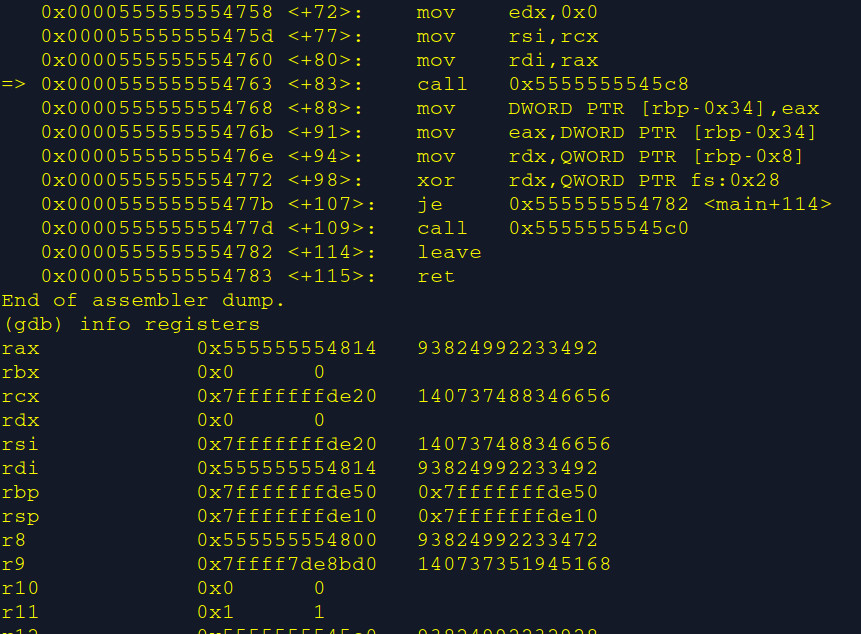
\includegraphics[width=15cm]{../images/Bufferoverflow_Aufgabe1a_Reg_b4_call.jpg}
	\caption{Aufgabe 1a Inhalt Register vor Call Execve()}
\end{figure}


\newpage

Im Register rdi befindet sich durch 
Zeile 
\begin{lstlisting}
0x0000555555554760 <+80>:   mov rdi, rax
\end{lstlisting}
die Adresse 0x555555554814 in der sich der String "/bin/sh" befindet. (siehe Abbildung 4)
\begin{lstlisting}
0x000055555555475d <+77>:   mov rsi, rcx
\end{lstlisting} 


Im Register rsi befindet sich die Adresse
des ersten Strings unserers Stringarrays cmd.
Die Adresse lautet 0x7fffffffde20. 
Diese Adresse liegt im Stack. 
Der Stack sieht vor dem Aufruf der Funktion folgendermaßen aus.

\begin{figure}[h!]
	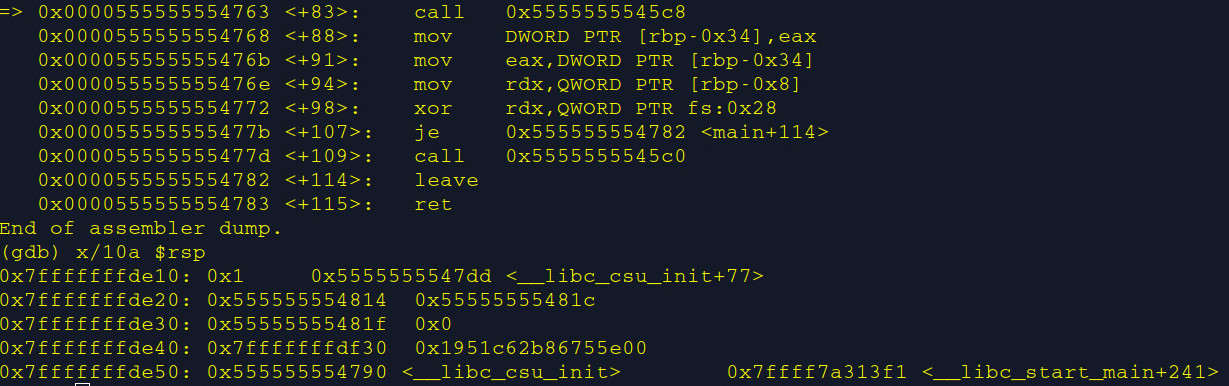
\includegraphics[width=15cm]{../images/Bufferoverflow_Aufgabe1a_StackVorCallExecve.jpg}
	\caption{Aufgabe 1a Inhalt Stack vor Aufruf execve()}
\end{figure}



\begin{lstlisting}
0x7fffffffde20: 0x555555554814  -> "/bin/sh"
0x7fffffffde28: 0x55555555481c	-> "-c"
0x7fffffffde30: 0x55555555481f	-> "ls -l"
0x7fffffffde38: 0x0
\end{lstlisting}
\begin{figure}[h!]
	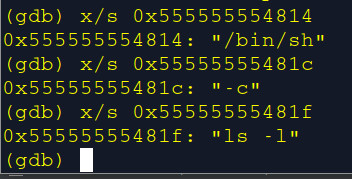
\includegraphics[width=5cm]{../images/Bufferoverflow_Aufgabe1a_Pointeruebergabeparams.jpg}
	\caption{Speicherort der Strings}
\end{figure}
Somit wird über den Register rsi das Stringarrays cmd übergeben.

\newpage
\begin{lstlisting}
0x0000555555554758 <+72>:    mov eax, 0x0 
\end{lstlisting}
Ist ein NULL, welches das dritte Übergabeparameter von execve ist.




\subsubsection{Wie und an welcher Stelle werden die übergebenen Parameter im Speicher abgelegt?}

Zunächst werden Pointer für alle Strings auf den Stack geschrieben um dann vor Funktionsaufruf in den entsprechenden Registern gespeichert zu werden.

Dump of assembler code for function main:
\begin{lstlisting}
   0x0000555555554710 <+0>:	push rbp
   0x0000555555554711 <+1>:	mov  rbp,rsp
   0x0000555555554714 <+4>:	sub  rsp,0x40
   0x0000555555554718 <+8>:	mov  rax,QWORD PTR fs:0x28
   0x0000555555554721 <+17>:mov  QWORD PTR [rbp-0x8],rax
   0x0000555555554725 <+21>:xor  eax,eax
   0x0000555555554727 <+23>:lea  rax,[rip+0xe6]
   0x000055555555472e <+30>:mov  QWORD PTR [rbp-0x30],rax
   0x0000555555554732 <+34>:lea  rax,[rip+0xe3]
   0x0000555555554739 <+41>:mov  QWORD PTR [rbp-0x28],rax
   0x000055555555473d <+45>:lea  rax,[rip+0xdb]
   0x0000555555554744 <+52>:mov  QWORD PTR [rbp-0x20],rax
   0x0000555555554748 <+56>:mov  QWORD PTR [rbp-0x18],0x0
   0x0000555555554750 <+64>:mov  rax,QWORD PTR [rbp-0x30]
   0x0000555555554754 <+68>:lea  rcx,[rbp-0x30]
   0x0000555555554758 <+72>:mov  edx,0x0
   0x000055555555475d <+77>:mov  rsi,rcx
   0x0000555555554760 <+80>:mov  rdi,rax
   0x0000555555554763 <+83>:call 0x5555555545c8
   0x0000555555554768 <+88>:mov  DWORD PTR [rbp-0x34],eax
   0x000055555555476b <+91>:mov  eax,DWORD PTR [rbp-0x34]
   0x000055555555476e <+94>:mov  rdx,QWORD PTR [rbp-0x8]
   0x0000555555554772 <+98>:xor  rdx,QWORD PTR fs:0x28
   0x000055555555477b <+107>:je 0x555555554782 <main+114>
   0x000055555555477d <+109>:call 0x5555555545c0
   0x0000555555554782 <+114>:leave  
   0x0000555555554783 <+115>:ret  
\end{lstlisting}
\newpage
Siehe Abbildung 3 für den Inhalt des Stacks, dieser reicht von der Adresse des Registers rbp(0x7fffffffde50) bis rsp(0x7fffffffde10)
+23 Pointer von "/bin/sh" wird in Register rax geschrieben \\
+30 Pointer von "/bin/sh" wird aus rax auf den Stack Addr: rbp-0x30 geschrieben\\
+34 Pointer von "-c" wird in rax geschrieben\\
+41 Pointer von "-c" wird aus Register rax auf den Stack Addr: rbp-0x28 geschrieben\\
+45 Pointer von "ls -l" wird in Register rax geschrieben\\
+52 Pointer von "ls -l" wird aus Register rax auf den Stack Addr: rbp-0x20 geschrieben\\
+56 Die folgenden 8 Byte auf dem Stack werden mit 0 beschrieben.\\
+64 Der Pointer auf den String "/bin/sh" wird aus dem Stack in den Register rax geschrieben.\\
+68 Die Adresse rbp-0x30 wird in den rsi geschrieben, diese Adresse zeigt auf den Stack und somit auf den Begin des Stringarrays.\\
+72	0 wird in Register rdx gespeichert.\\
+77 Pointer der auf den Beginn des Stringarrays im Stack zeigt wird in rsi gespeichert.\\ 
+80 Pointer auf den String "bin/sh" wird in Register rdi gespeichert.\\

Im Stack werden die Stringadressen als QWORD Pointer gespeichert, d.h 8byte pointer =64bit



\newpage
\subsubsection{Welche Daten befinden sich beim Aufruf von execve() im Stack Frame?}
Im Stack befindet sich die Rücksprungadresse auf die mainfunktion

\begin{figure}[h!]
	\includegraphics[width=10cm]{../images/Bildschirmfoto_rücksprungadresseimstack.jpg}
	\caption{neuer Stackframe beim aufruf von execve()}
\end{figure}

\begin{lstlisting}
(gdb) x/a $rsp
0x7fffffffde08:	0x555555554768 <main+88>
\end{lstlisting}
0x555555554768
ist die Adresse die der rip nach ausführen der funktion execve wieder aufnehmen muss,
dies ist der nächste Befehl nach Aufruf der Funktion execve() in der Mainfunktion
\begin{lstlisting}
0x0000555555554763 <+83>:call 0x5555555545c8
0x0000555555554768 <+88>:mov  DWORD PTR [rbp-0x34],eax
0x000055555555476b <+91>:mov  eax,DWORD PTR [rbp-0x34]
0x000055555555476e <+94>:mov  rdx,QWORD PTR [rbp-0x8]
0x0000555555554772 <+98>:xor  rdx,QWORD PTR fs:0x28
0x000055555555477b <+107>:je   0x555555554782 <main+114>
0x000055555555477d <+109>:call 0x5555555545c0
0x0000555555554782 <+114>:leave  
0x0000555555554783 <+115>:ret    
\end{lstlisting}






\end{document}


